\documentclass{beamer}
\usepackage[utf8]{inputenc}

\usetheme{Madrid}
\usecolortheme{default}
\usepackage{amsmath,amssymb,amsfonts,amsthm}
\usepackage{txfonts}
\usepackage{tkz-euclide}
\usepackage{listings}
\usepackage{adjustbox}
\usepackage{array}
\usepackage{tabularx}
\usepackage{gvv}
\usepackage{lmodern}
\usepackage{circuitikz}
\usepackage{tikz}
\usepackage{graphicx}
\usepackage{mathtools}
\setbeamertemplate{page number in head/foot}[totalframenumber]

\usepackage{tcolorbox}
\tcbuselibrary{minted,breakable,xparse,skins}



\definecolor{bg}{gray}{0.95}
\DeclareTCBListing{mintedbox}{O{}m!O{}}{%
  breakable=true,
  listing engine=minted,
  listing only,
  minted language=#2,
  minted style=default,
  minted options={%
    linenos,
    gobble=0,
    breaklines=true,
    breakafter=,,
    fontsize=\small,
    numbersep=8pt,
    #1},
  boxsep=0pt,
  left skip=0pt,
  right skip=0pt,
  left=25pt,
  right=0pt,
  top=3pt,
  bottom=3pt,
  arc=5pt,
  leftrule=0pt,
  rightrule=0pt,
  bottomrule=2pt,
  toprule=2pt,
  colback=bg,
  colframe=orange!70,
  enhanced,
  overlay={%
    \begin{tcbclipinterior}
    \fill[orange!20!white] (frame.south west) rectangle ([xshift=20pt]frame.north west);
    \end{tcbclipinterior}},
  #3,
}
\lstset{
    language=C,
    basicstyle=\ttfamily\small,
    keywordstyle=\color{blue},
    stringstyle=\color{orange},
    commentstyle=\color{green!60!black},
    numbers=left,
    numberstyle=\tiny\color{gray},
    breaklines=true,
    showstringspaces=false,
}

\title 
{1.10.11}
\date{September, 2025}


\author 
{Surya Sri - EE25BTECH11053}



\begin{document}


\frame{\titlepage}
\begin{frame}{Question}
Find a vector of magnitude 5 units, and parallel to the resultant of the vectors $\vec{a} = 2\hat{i} + 3\hat{j} - \hat{k}$ and $\vec{b} = \hat{i} - 2\hat{j} + \hat{k}$.
\end{frame}



\begin{frame}{Variables used}
\begin{table}[H]    
  \centering
  \begin{tabular}[12pt]{ |c| c|}
    \hline
    \textbf{Point} & \textbf{Vector}\\ 
    \hline
    $\mathbf{v_1}$ &  $\myvec{1\\1\\1}$\\
    \hline
    $\mathbf{v_2}$ &   $\myvec{1\\-1\\1}$\\
    \hline
     $\mathbf{v_3}$ &  $\myvec{1\\1\\-1}$\\
    \hline
    \end{tabular}
  \caption{Variables Used}
  \label{tab:1.5.39}
\end{table}

\end{frame}

\begin{frame}{Solution}
Let the required vector be $\vec{R}$ ,

\begin{align}
    \vec{R} = k(\vec{a} + \vec{b})
\end{align}

Magnitude of Resultant vector is,
\begin{align}
\norm{R} = \sqrt{3^2 + 1^2 + 0^2} = \sqrt{9 + 1} = \sqrt{10}
\end{align}

Let the desired vector be,
\begin{align}
    \norm{k\vec{R}} = 5
\end{align}

\begin{align}
     |{k}|\sqrt{10} = 5 
\end{align}  

\begin{align}
\implies k = \frac{5}{\sqrt{10}}
\end{align}
 
\end{frame}

\begin{frame}{Solution}
\begin{align}
\vec{a} + \vec{b} = \begin{pmatrix} 3 \\ 1 \\ 0 \end{pmatrix}
\end{align}

So,
\begin{align}
\boxed{
\vec{R} = \frac{5}{\sqrt{10}}
\begin{pmatrix}
3 \\
1 \\
0
\end{pmatrix}
}
\end{align}
    
\begin{align}
\vec{R} = \begin{bmatrix}
\frac{15}{\sqrt{10}} \\
\frac{5}{\sqrt{10}} \\
0
\end{bmatrix}
\end{align}
is a matrix with magnitude 5 parallel to the resultant vector.





\end{frame}


\begin{frame}[fragile]
    \frametitle{Python}
    \begin{lstlisting}

import matplotlib.pyplot as plt
import numpy as np

# Define vectors
a = np.array([2, 3, -1])
b = np.array([1, -2, 1])

# Resultant vector: a + b
r = a + b

# Magnitude of resultant
mag_r = np.linalg.norm(r)

# Unit vector in direction of resultant
unit_r = r / mag_r



\end{lstlisting}
\end{frame}


\begin{frame}[fragile]
    \frametitle{Python}
    \begin{lstlisting}    
# Vector of magnitude 5, parallel to r
res = 5 * unit_r

fig = plt.figure()
ax = fig.add_subplot(111, projection='3d')
# Origin
origin = np.array([0, 0, 0])

# Plot vectors
ax.quiver(*origin, *a, color='r', label='a', linewidth=2)
ax.quiver(*origin, *b, color='g', label='b', linewidth=2)
ax.quiver(*origin, *res, color='b', label='Resultant (Mag 5)', linewidth=2)





\end{lstlisting}
\end{frame}



\begin{frame}[fragile]
    \frametitle{Python}
    \begin{lstlisting}
# Axes labels
ax.set_xlim([0, 5])
ax.set_ylim([0, 5])
ax.set_zlim([-2, 2])
ax.set_xlabel('X')
ax.set_ylabel('Y')
ax.set_zlabel('Z')

# Add legend
ax.legend()

plt.title('graph')
plt.savefig("graph.png") 
plt.show()


\end{lstlisting}
\end{frame}


\begin{frame}[fragile]
\frametitle{C Code}
\begin{lstlisting}
  
#include <stdio.h>
#include <math.h>

int main() {
    // Given vectors
    double a[3] = {2, 3, -1};
    double b[3] = {1, -2, 1};
    double r[3], mag_r, unit_r[3], result[3];
    int i;

    // Calculate resultant r = a + b
    for(i = 0; i < 3; i++)
        r[i] = a[i] + b[i];


 \end{lstlisting}
\end{frame} 


\begin{frame}[fragile]
\frametitle{C Code}
\begin{lstlisting}
    
    // Magnitude of r
    mag_r = sqrt(r[0]*r[0] + r[1]*r[1] + r[2]*r[2]);

    // Unit vector in direction of r
    for(i = 0; i < 3; i++)
        unit_r[i] = r[i] / mag_r;

    // Vector of magnitude 5, parallel to r
    for(i = 0; i < 3; i++)
        result[i] = 5 * unit_r[i];

    // Print result
    printf("Vector of magnitude 5, parallel to resultant: ");
    printf("(%.4lf) i + (%.4lf) j + (%.4lf) k\n", result[0], result[1], result[2]);

    return 0;
     }

\end{lstlisting}
\end{frame}

\begin{frame}[fragile]
\frametitle{Python and C Code}

\begin{lstlisting}
 import subprocess

# Compile the C program
subprocess.run(["gcc", "points.c", "-o", "points"])

# Run the compiled C program
result = subprocess.run(["./points"], capture_output=True, text=True)

# Print the output from the C program (solution)
print(result.stdout) 

\end{lstlisting}
\end{frame}


\begin{frame}[fragile]
\frametitle{Graph}

\begin{figure}[H]
\begin{center}
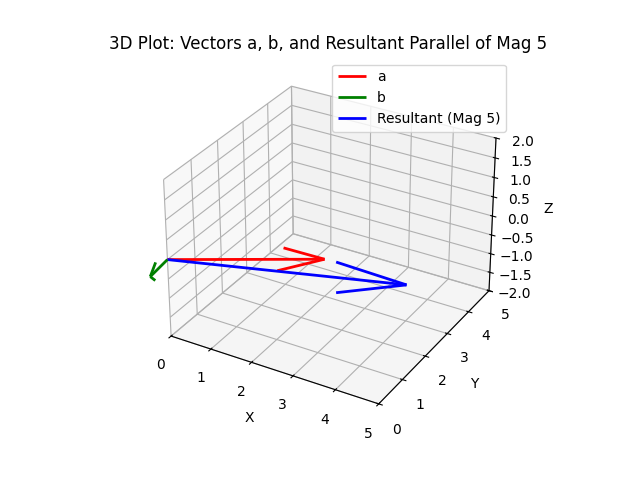
\includegraphics[width=0.75\columnwidth]{../figs/graph.png}
\end{center}
\caption{}
\label{fig:Fig}
\end{figure}




\end{frame}



\end{document}